\begin{figure}[ht]
\vskip 0.05in
\begin{center}
\centerline{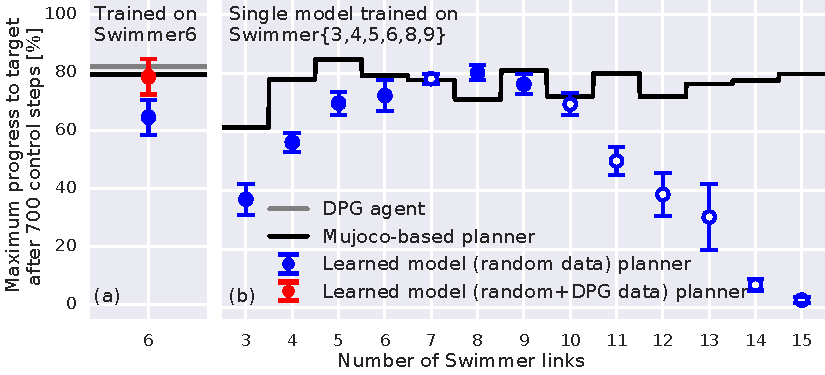
\includegraphics[width=\columnwidth]{figures/control_swimmer_comparison_full}}
\vspace{-0.1in}
\caption{GN-based MPC performance (\% distance to target after 700 steps) for (a) model trained on Swimmer6 and (b) model trained on Swimmers with 3-15 links (see Figure~\ref{fig:multiple_swimmer_rollout_baseline}). In (a), GN-based MPC (blue point) is almost as good as the Mujoco-based planner (black line) and trained DDPG (grey line) baselines. When the GN-based MPC's model is trained on a mixture of random and DDPG agent Swimmer6 trajectories (red point), its performance is as good as the strong baselines. In (b) the GN-based MPC (blue point) (video: \href{\controlmultipleswimmer}{\controlmultipleswimmername}) is competitive with a Mujoco-based planner baseline (black) (video: \href{\controlmultipleswimmerbaseline}{\controlmultipleswimmerbaselinename}) for 6-10 links, but is worse for 3-5 and 11-15 links. Note, the model was not trained on the open points, 7 and 10-15 links, which correspond to zero-shot model generalization for control. Error bars indicate mean and standard deviation across 5 experimental runs.
}
\label{fig:control_swimmer_comparison_full}
\end{center}
\vskip -0.2in
\end{figure}